\chapter{DỮ LIỆU VÀ PHƯƠNG PHÁP}
\label{ch:phuong_phap}

\section{Bộ dữ liệu}

\subsection{Nguồn và quy mô}

Đề tài sử dụng bộ dữ liệu \textit{pkdarabi/cardetection} công bố trên Kaggle, phân phối dưới dạng
một bản xuất Roboflow theo bố cục thư mục chuẩn \texttt{\{train,valid,test\}/\{images,labels\}}
với nhãn ở định dạng YOLO TXT. Mặc dù tên trên đường dẫn là ``car detection'', nội dung thực tế
của toàn bộ 15 lớp đều là đèn tín hiệu và biển giới hạn tốc độ, không có lớp nào là phương tiện.
Nhóm thực hiện giữ nguyên 15 lớp gốc, không gộp cũng không ánh xạ lại nhãn, để kết quả có thể đối
chiếu với các công bố khác dùng cùng bộ dữ liệu.

Một quyết định thiết kế đáng nói ở đây: mô-đun kiểm tra dữ liệu được viết để \emph{tự phát hiện}
định dạng chú thích thay vì giả định sẵn. Hàm dò tìm sẽ lần lượt kiểm tra sự tồn tại của tệp
\texttt{.txt} kèm \texttt{data.yaml}, rồi tới \texttt{.json}, \texttt{.xml} và \texttt{.csv} để
kết luận bộ dữ liệu đang ở định dạng YOLO, COCO, VOC hay CSV. Cách làm này bảo đảm báo cáo mô tả
đúng dữ liệu thật chứ không mô tả giả định của người viết.

\begin{table}[H]
\centering
\caption{Thống kê tổng quan bộ dữ liệu theo từng tập}
\label{tab:dataset_summary}
\small
\begin{tabular}{lrrrr}
\toprule
\textbf{Tập} & \textbf{Số ảnh} & \textbf{Tỉ lệ} & \textbf{Số hộp bao} & \textbf{Hộp/ảnh} \\
\midrule
Huấn luyện & 3.530 & 71,0\% & 4.298 & 1,218 \\
Kiểm định  & 801   & 16,1\% & 944   & 1,179 \\
Kiểm tra   & 638   & 12,8\% & 770   & 1,207 \\
\midrule
\textbf{Tổng} & \textbf{4.969} & \textbf{100\%} & \textbf{6.012} & \textbf{1,210} \\
\bottomrule
\end{tabular}
\end{table}

Toàn bộ ảnh có độ phân giải đồng nhất 416$\times$416 điểm ảnh --- hệ quả của bước tiền xử lý mà
Roboflow áp dụng khi xuất bộ dữ liệu. Chi tiết này tưởng nhỏ nhưng có hai hệ quả kỹ thuật quan
trọng sẽ được bàn ở Mục~\ref{sec:thanhphan}: nó khiến việc tăng kích thước ảnh đầu vào khi huấn
luyện không bổ sung thêm chi tiết thật, và nó khiến mọi ảnh trong một lô có cùng kích thước nên
bước đệm trong nhánh DETR không bao giờ được kích hoạt.

Mật độ vật thể rất thưa: trung bình chỉ 1,21 hộp bao trên mỗi ảnh, cao nhất là 10 hộp ở tập kiểm
tra. Đây là đặc điểm khác hẳn các bộ dữ liệu cảnh đường phố như TT100K~\cite{zhu2016tt100k}, nơi
một khung hình có thể chứa hàng chục biển báo.

\subsection{Phân bố lớp và mất cân bằng}

\begin{figure}[H]
\centering
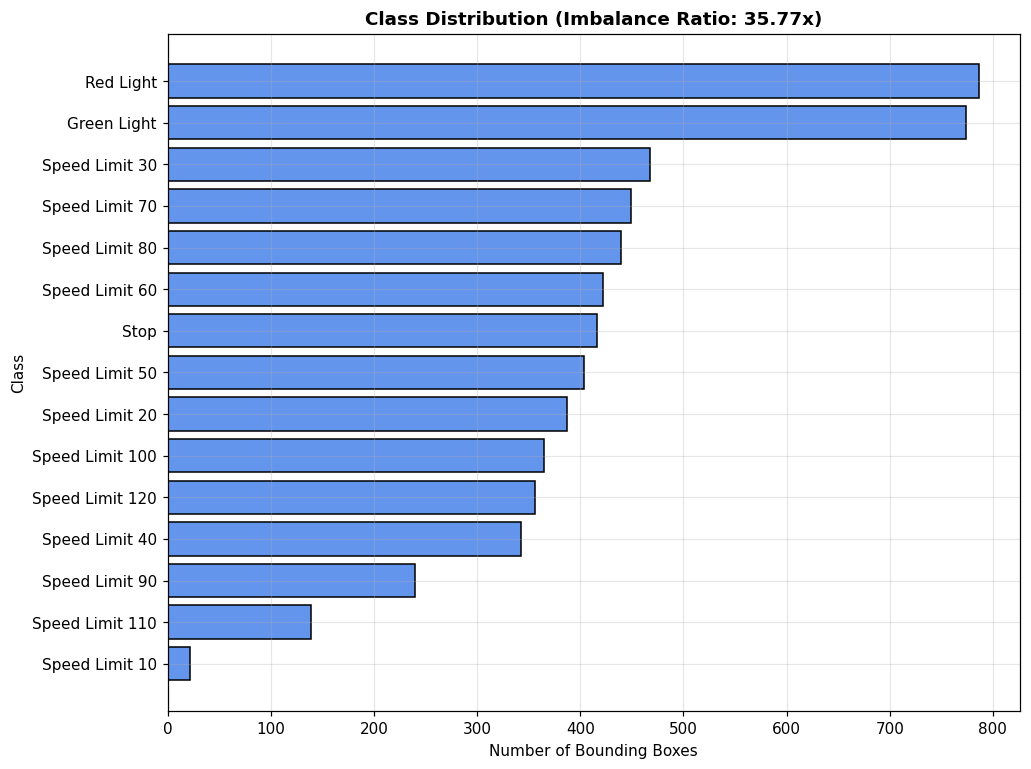
\includegraphics[width=0.92\textwidth]{figures/eda_class_distribution.png}
\caption{Phân bố số hộp bao theo từng lớp trên toàn bộ dữ liệu}
\label{fig:class_dist}
\end{figure}

Hình~\ref{fig:class_dist} và Bảng~\ref{tab:class_dist} cho thấy mức mất cân bằng đáng kể. Hai lớp
đèn tín hiệu chiếm gần 26\% tổng số hộp bao, trong khi lớp \textit{Speed Limit 10} chỉ có 22 mẫu,
tương đương 0,37\%. Tỉ số mất cân bằng, định nghĩa bằng thương giữa số mẫu của lớp nhiều nhất và
lớp ít nhất, đạt \textbf{35,77}.

\begin{table}[H]
\centering
\caption{Phân bố lớp chi tiết, sắp theo số hộp bao giảm dần}
\label{tab:class_dist}
\small
\begin{tabular}{clrrr}
\toprule
\textbf{Mã lớp} & \textbf{Tên lớp} & \textbf{Số hộp} & \textbf{Tỉ lệ (\%)} & \textbf{Tỉ số so với lớp lớn nhất} \\
\midrule
1  & Red Light        & 787 & 13,09 & 1,00 \\
0  & Green Light      & 774 & 12,87 & 1,02 \\
7  & Speed Limit 30   & 468 & 7,78  & 1,68 \\
11 & Speed Limit 70   & 449 & 7,47  & 1,75 \\
12 & Speed Limit 80   & 440 & 7,32  & 1,79 \\
10 & Speed Limit 60   & 422 & 7,02  & 1,86 \\
14 & Stop             & 416 & 6,92  & 1,89 \\
9  & Speed Limit 50   & 404 & 6,72  & 1,95 \\
6  & Speed Limit 20   & 387 & 6,44  & 2,03 \\
3  & Speed Limit 100  & 365 & 6,07  & 2,16 \\
5  & Speed Limit 120  & 356 & 5,92  & 2,21 \\
8  & Speed Limit 40   & 343 & 5,71  & 2,29 \\
13 & Speed Limit 90   & 240 & 3,99  & 3,28 \\
4  & Speed Limit 110  & 139 & 2,31  & 5,66 \\
2  & Speed Limit 10   & 22  & 0,37  & \textbf{35,77} \\
\bottomrule
\end{tabular}
\end{table}

Khi cài đặt phép tính này, một chi tiết dễ sai đã được xử lý tường minh: nếu chỉ đếm các lớp thực
sự xuất hiện trong dữ liệu, một lớp được khai báo trong tệp cấu hình nhưng không có mẫu nào sẽ bị
âm thầm bỏ qua, khiến tỉ số mất cân bằng bị báo cáo thấp hơn thực tế và ``lớp hiếm nhất'' bị xác
định sai. Mô-đun phân tích do đó đánh chỉ mục lại bảng đếm theo toàn bộ tập lớp khai báo với giá
trị mặc định bằng không, và trả về vô cùng khi có lớp rỗng.

\subsection{Thống kê kích thước hộp bao}

\begin{figure}[H]
\centering
\begin{subfigure}[b]{0.48\textwidth}
  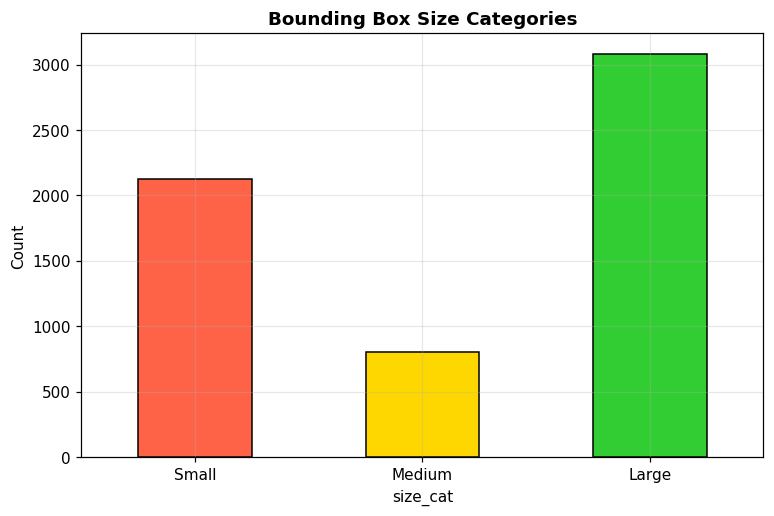
\includegraphics[width=\textwidth]{figures/eda_bbox_size_categories.png}
  \caption{Phân nhóm kích thước}
\end{subfigure}
\hfill
\begin{subfigure}[b]{0.48\textwidth}
  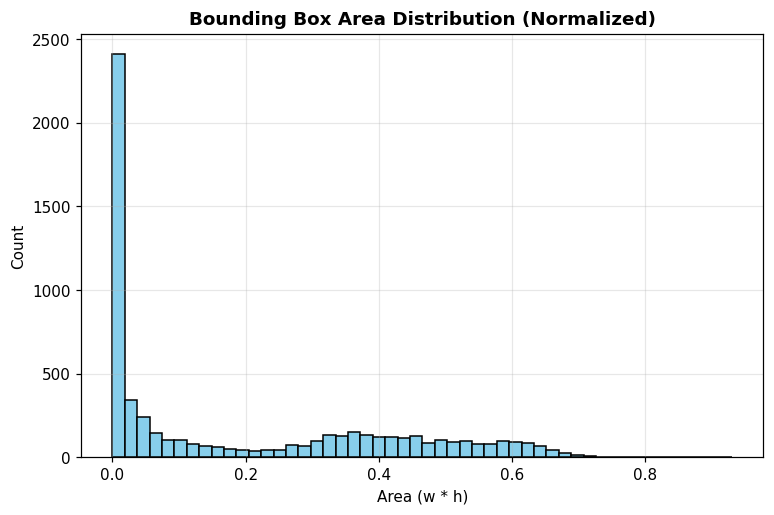
\includegraphics[width=\textwidth]{figures/eda_bbox_area.png}
  \caption{Phân bố diện tích chuẩn hoá}
\end{subfigure}
\caption{Thống kê kích thước hộp bao trên toàn bộ dữ liệu}
\label{fig:bbox_size}
\end{figure}

Việc phân nhóm kích thước dùng diện tích đã chuẩn hoá $a = w \cdot h$ với $w, h \in [0,1]$, theo
ba ngưỡng: nhỏ khi $a < 0{,}01$, trung bình khi $0{,}01 \le a < 0{,}05$, và lớn trong các trường
hợp còn lại. Cần lưu ý rằng quy ước này khác với quy ước COCO~\cite{lin2014coco}, vốn dùng diện
tích tuyệt đối theo điểm ảnh với các ngưỡng $32^2$ và $96^2$. Lựa chọn dùng diện tích chuẩn hoá là
có chủ ý: nó độc lập với độ phân giải ảnh nên so sánh được giữa các nguồn dữ liệu khác nhau.

\begin{table}[H]
\centering
\caption{Phân nhóm kích thước hộp bao theo diện tích chuẩn hoá}
\label{tab:bbox_cat}
\small
\begin{tabular}{lrrl}
\toprule
\textbf{Nhóm} & \textbf{Số hộp} & \textbf{Tỉ lệ (\%)} & \textbf{Ngưỡng diện tích chuẩn hoá} \\
\midrule
Nhỏ        & 2.122 & 35,30 & $a < 0{,}01$ \\
Trung bình & 806   & 13,41 & $0{,}01 \le a < 0{,}05$ \\
Lớn        & 3.084 & 51,30 & $a \ge 0{,}05$ \\
\bottomrule
\end{tabular}
\end{table}

Bảng~\ref{tab:bbox_cat} chứa một tín hiệu bất thường. Trong một bộ dữ liệu cảnh đường phố thông
thường, nhóm vật thể lớn hiếm khi chiếm quá bán, bởi biển báo chiếm hơn 5\% diện tích khung hình
đồng nghĩa với việc xe đã ở rất gần biển. Ở đây nhóm lớn chiếm tới 51,30\%. Điều này thúc đẩy phân
tích ở mục tiếp theo.

\subsection{Phân tích thành phần bộ dữ liệu}
\label{sec:thanhphan}

Quan sát tên tệp cho thấy bộ dữ liệu không đồng nhất mà là một tập \emph{trộn} từ nhiều nguồn có
quy ước đặt tên khác nhau. Nhóm thực hiện phân loại ảnh theo mẫu tên tệp và tính lại thống kê kích
thước riêng cho từng nhóm; kết quả trình bày ở Bảng~\ref{tab:thanhphan}.

\begin{table}[H]
\centering
\caption{Thành phần bộ dữ liệu theo nguồn gốc suy ra từ quy ước đặt tên tệp}
\label{tab:thanhphan}
\small
\begin{tabular}{lrrrr}
\toprule
\textbf{Nhóm nguồn} & \textbf{Số ảnh} & \textbf{Tỉ lệ (\%)} & \textbf{Cạnh biển (trung vị)} & \textbf{\% vật thể nhỏ} \\
\midrule
Ảnh cắt kiểu GTSRB & 1.922 & 38,68 & 66,8\% cạnh ảnh & 0,0 \\
Ảnh số sáu chữ số  & 1.586 & 31,92 & 19,6\%          & 34,7 \\
Ảnh cảnh đường     & 724   & 14,57 & 13,4\%          & 31,1 \\
Camera mắt cá      & 645   & 12,98 & 1,6\%           & 99,6 \\
Nhóm khác          & 92    & 1,85  & 75,7\%          & 0,0 \\
\bottomrule
\end{tabular}
\end{table}

Kết quả này giải thích trọn vẹn hình dạng bất thường ở Bảng~\ref{tab:bbox_cat}. Nhóm ảnh cắt kiểu
GTSRB chiếm 38,68\% số ảnh và có biển báo lấp gần kín khung hình --- đây vốn là ảnh dành cho bài
toán \emph{phân lớp} chứ không phải \emph{phát hiện}~\cite{stallkamp2012gtsrb}. Ở đầu kia của
thang đo, nhóm camera mắt cá có tới 99,6\% vật thể thuộc nhóm nhỏ, với cạnh biển trung vị chỉ
1,6\% cạnh ảnh, đồng thời mang hình học quang học hoàn toàn khác.

Hệ quả là phân bố kích thước bị \emph{lưỡng cực}. Bảng~\ref{tab:percentile} trình bày các phân vị
diện tích quy đổi ra cạnh tính bằng điểm ảnh trên ảnh 416$\times$416.

\begin{table}[H]
\centering
\caption{Phân vị diện tích hộp bao và cạnh tương ứng trên ảnh 416$\times$416}
\label{tab:percentile}
\small
\begin{tabular}{lrrrrr}
\toprule
\textbf{Phân vị} & \textbf{10\%} & \textbf{25\%} & \textbf{50\%} & \textbf{75\%} & \textbf{90\%} \\
\midrule
Diện tích chuẩn hoá & 0,0003 & 0,0025 & 0,0570 & 0,3854 & 0,5402 \\
Cạnh tương ứng (điểm ảnh) & 6,9 & 20,8 & 99,3 & 258,2 & 305,8 \\
\bottomrule
\end{tabular}
\end{table}

Khoảng cách giữa phân vị 25\% (20,8 điểm ảnh) và phân vị 75\% (258,2 điểm ảnh) là hơn mười hai
lần, và vùng ``biển báo thật trên đường'' --- khoảng 30 đến 80 điểm ảnh --- gần như trống. Nói cách
khác, mô hình được dạy chủ yếu bằng hai chế độ cực đoan mà thiếu hẳn chế độ trung gian vốn là chế
độ thường gặp nhất trong thực tế. Đây là một dạng thiên lệch bộ dữ liệu điển
hình~\cite{torralba2011bias} và là chìa khoá để diễn giải kết quả ở Chương~\ref{ch:ket_qua}.

\begin{figure}[H]
\centering
\begin{subfigure}[b]{0.32\textwidth}
  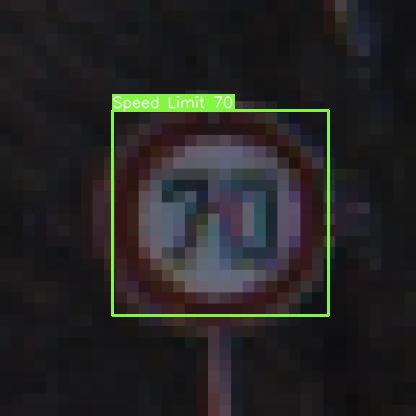
\includegraphics[width=\textwidth]{figures/sample_gtsrb_crop.jpg}
  \caption{Ảnh cắt kiểu GTSRB}
\end{subfigure}
\hfill
\begin{subfigure}[b]{0.32\textwidth}
  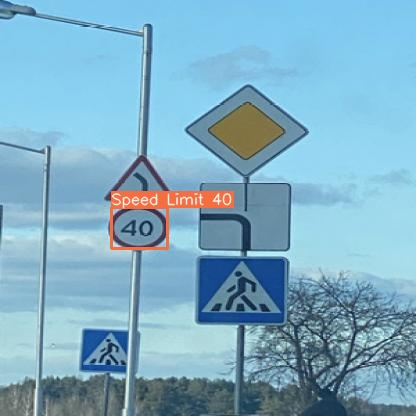
\includegraphics[width=\textwidth]{figures/sample_road_scene.jpg}
  \caption{Ảnh cảnh đường}
\end{subfigure}
\hfill
\begin{subfigure}[b]{0.32\textwidth}
  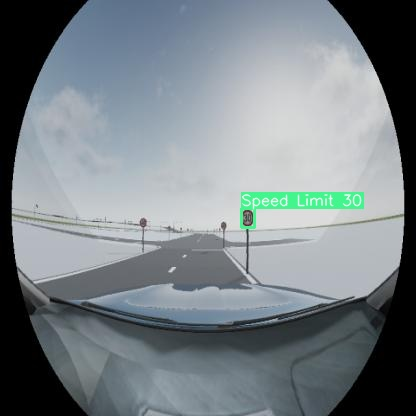
\includegraphics[width=\textwidth]{figures/sample_fisheye.jpg}
  \caption{Camera mắt cá}
\end{subfigure}
\caption{Ba chế độ ảnh cùng tồn tại trong bộ dữ liệu, kèm hộp bao nhãn thật}
\label{fig:ba_che_do}
\end{figure}

\subsection{Vị trí vật thể trong khung hình}

\begin{figure}[H]
\centering
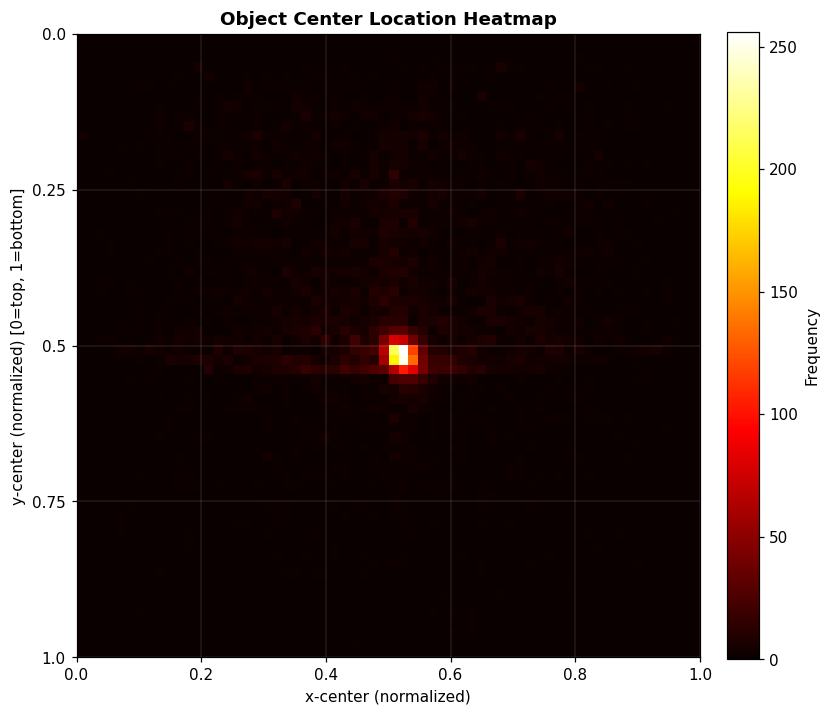
\includegraphics[width=0.62\textwidth]{figures/eda_object_center_heatmap.png}
\caption{Bản đồ nhiệt vị trí tâm vật thể trên toàn bộ dữ liệu}
\label{fig:heatmap}
\end{figure}

Bản đồ nhiệt ở Hình~\ref{fig:heatmap} được xây bằng biểu đồ tần suất hai chiều trên toạ độ tâm đã
chuẩn hoá. Hai chi tiết cài đặt cần lưu ý. Thứ nhất, trục tung được lật theo phép $y' = 1 - y_c$
vì hệ toạ độ ảnh đặt gốc ở góc trên trái với trục $y$ hướng xuống, trong khi hệ toạ độ đồ thị
hướng lên. Thứ hai, ma trận tần suất phải được chuyển vị trước khi hiển thị, do hàm dựng biểu đồ
hai chiều trả về theo thứ tự (trục hoành, trục tung) còn hàm hiển thị ảnh yêu cầu thứ tự (hàng,
cột). Bỏ qua một trong hai bước này sẽ cho một bản đồ nhiệt trông hợp lý nhưng sai hoàn toàn về
mặt hình học.

\subsection{Kiểm tra chất lượng nhãn}

Một mô-đun kiểm tra độc lập rà soát tám loại lỗi: thiếu ảnh, thiếu nhãn, nhãn rỗng, ảnh hỏng, trùng
tên ảnh giữa các tập, mã lớp ngoài miền hợp lệ, toạ độ hộp nằm ngoài đoạn $[0,1]$ và hộp có cạnh
bằng không. Kết quả trên bộ dữ liệu thật ghi nhận \textbf{4 ảnh có tệp nhãn rỗng}, tức ảnh nền
không chứa biển báo nào. Đây không phải lỗi mà là ảnh nền hợp lệ, thường được giữ lại có chủ đích
để giảm dương tính giả.

Về mặt cài đặt, việc đối chiếu tên ảnh với tên tệp nhãn dùng cấu trúc tập hợp thay vì danh sách,
nhờ đó phép kiểm tra thành viên có độ phức tạp hằng số thay vì tuyến tính, tránh chi phí bậc hai
khi quy mô dữ liệu tăng.

\section{Kiến trúc quy trình}

Toàn bộ mã nguồn được tổ chức thành các gói độc lập, mỗi gói chịu trách nhiệm một giai đoạn của
quy trình, và sổ tay Jupyter chỉ đóng vai trò điều phối. Bảng~\ref{tab:modules} tóm tắt.

\begin{table}[H]
\centering
\caption{Tổ chức mô-đun của quy trình}
\label{tab:modules}
\small
\begin{tabular}{p{4.2cm} p{9.3cm}}
\toprule
\textbf{Gói} & \textbf{Chức năng} \\
\midrule
\texttt{src/utils}      & Đăng ký đường dẫn tập trung, tiện ích vẽ đồ thị, gieo hạt bộ sinh ngẫu nhiên \\
\texttt{src/data}       & Dò định dạng, kiểm tra chất lượng nhãn, trực quan hoá chú thích, chuyển YOLO sang COCO \\
\texttt{src/eda}        & Phân bố lớp, thống kê hộp bao, thống kê ảnh, bản đồ nhiệt vị trí \\
\texttt{src/training}   & Huấn luyện YOLO và DETR \\
\texttt{src/evaluation} & Đánh giá độ chính xác, đo tốc độ, tổng hợp bảng so sánh \\
\texttt{tests}          & 43 trường hợp kiểm thử chạy trên CPU trong khoảng một giây \\
\bottomrule
\end{tabular}
\end{table}

\subsection{Bảo đảm tính tái lập}

Ba biện pháp được áp dụng. Thứ nhất, một hàm gieo hạt duy nhất đặt hạt cho biến môi trường băm
của Python, thư viện ngẫu nhiên chuẩn, NumPy, PyTorch và PyTorch CUDA, đồng thời bật chế độ tất
định của cuDNN và \emph{tắt} chế độ tự dò thuật toán nhanh nhất. Việc tắt chế độ tự dò là cần
thiết vì nó chọn thuật toán tích chập theo điều kiện thực thi tại thời điểm chạy, khiến kết quả
không lặp lại được giữa các lần. Hạt mặc định là 42 và được truyền tường minh vào cả bộ huấn luyện
của Ultralytics.

Thứ hai, mọi đường dẫn đầu vào và đầu ra được khai báo tại một mô-đun duy nhất, có hỗ trợ biến môi
trường để cùng một mã nguồn chạy được trên máy cá nhân lẫn trên Colab với dữ liệu đặt ở Google
Drive. Riêng tệp cấu hình dữ liệu của Ultralytics được sinh lại với đường dẫn tuyệt đối tại thời
điểm chạy, do thư viện này giải đường dẫn tương đối theo thư mục dữ liệu nội bộ của nó chứ không
theo thư mục dự án.

Thứ ba, các thư viện học sâu được nhập \emph{trễ}, tức chỉ nhập bên trong hàm cần dùng. Nhờ vậy
các mô-đun phân tích dữ liệu và bộ kiểm thử chạy được trên máy chỉ có CPU, không cần cài đặt
PyTorch~\cite{paszke2019pytorch} hay Ultralytics.

\section{Thiết kế thực nghiệm}

Bốn nhóm thực nghiệm được ký hiệu từ E0 đến E3, trình bày ở Bảng~\ref{tab:thietke}.

\begin{table}[H]
\centering
\caption{Thiết kế bốn nhóm thực nghiệm}
\label{tab:thietke}
\small
\begin{tabular}{p{1.1cm} p{5.0cm} p{7.4cm}}
\toprule
\textbf{Mã} & \textbf{Câu hỏi} & \textbf{Cấu hình khảo sát} \\
\midrule
E0 & Mốc so sánh là bao nhiêu? & YOLOv8n và DETR-ResNet50 \\
E1 & Có kiến trúc nhẹ nào không kém hơn? & YOLO11n, SSDLite-MobileNetV3, D-FINE-Nano \\
E2 & Nén được mô hình tốt nhất mà không huấn luyện lại không? & FP16, ONNX INT8, OpenVINO INT8 \\
E3 & Học trò nhỏ có học được từ thầy lớn không? & YOLO26s dạy YOLO26n \\
\bottomrule
\end{tabular}
\end{table}

\subsection{Cấu hình huấn luyện nhánh YOLO}

Mô hình nền là YOLOv8n, biến thể nhỏ nhất trong họ YOLOv8, khởi tạo từ trọng số tiền huấn luyện
trên COCO với 80 lớp; đầu phân loại được thay để khớp 15 lớp của đề tài. Bảng~\ref{tab:yolo_cfg}
liệt kê các siêu tham số chính, trích trực tiếp từ tệp tham số mà Ultralytics ghi lại sau khi
huấn luyện.

\begin{table}[H]
\centering
\caption{Siêu tham số huấn luyện YOLOv8n}
\label{tab:yolo_cfg}
\small
\begin{tabular}{lll}
\toprule
\textbf{Tham số} & \textbf{Giá trị} & \textbf{Ghi chú} \\
\midrule
Số chu kỳ        & 30      & Ngân sách cố định cho mọi cấu hình nhánh YOLO \\
Kích thước ảnh   & 640     & Cân bằng giữa tốc độ và độ chính xác \\
Kích thước lô    & 16      & \\
Hạt ngẫu nhiên   & 42      & Truyền tường minh vào bộ huấn luyện \\
Tốc độ học đầu   & 0,01    & Bộ tối ưu chọn tự động \\
Suy giảm trọng số& 0,0005  & \\
Chu kỳ khởi động & 3       & \\
Lật ngang        & \textbf{0,0} & \textbf{Tắt có chủ đích --- xem giải thích bên dưới} \\
Lật dọc          & 0,0     & \\
Ghép ảnh mosaic  & 1,0     & Tắt ở 10 chu kỳ cuối \\
Biến đổi tỉ lệ   & 0,5     & \\
Tịnh tiến        & 0,1     & \\
Nhiễu màu HSV    & 0,015 / 0,7 / 0,4 & Sắc độ / bão hoà / độ sáng \\
Xoá ngẫu nhiên   & 0,4     & \\
\bottomrule
\end{tabular}
\end{table}

Quyết định đáng chú ý nhất trong bảng trên là \textbf{tắt phép lật ngang}. Đây không phải giá trị
mặc định của thư viện mà là lựa chọn xuất phát từ đặc thù bài toán: nhiều biển báo giao thông mang
tính định hướng, chẳng hạn biển rẽ trái và biển rẽ phải chỉ khác nhau ở chiều mũi tên. Lật ngang
một ảnh chứa biển rẽ trái sẽ tạo ra hình ảnh của biển rẽ phải nhưng vẫn giữ nhãn cũ, tức là sinh
ra mẫu huấn luyện \emph{sai}. Đây là ví dụ cho nguyên tắc rằng tăng cường dữ liệu phải phù hợp với
ngữ nghĩa của miền ứng dụng chứ không thể áp dụng máy móc~\cite{shorten2019augmentation}.

Ngược lại, phép ghép ảnh mosaic được giữ ở hệ số tối đa. Kỹ thuật này, phổ biến từ
YOLOv4~\cite{bochkovskiy2020yolov4}, ghép bốn ảnh huấn luyện thành một, nhờ đó vừa tăng số ngữ
cảnh nền mà mỗi vật thể xuất hiện, vừa tạo ra các vật thể ở tỉ lệ nhỏ hơn --- đúng chế độ mà bộ dữ
liệu đang thiếu. Mosaic được tắt ở 10 chu kỳ cuối để mô hình kết thúc quá trình huấn luyện trên
phân bố ảnh gần với phân bố lúc suy luận.

\subsection{Cấu hình huấn luyện nhánh DETR}

Nhánh DETR tinh chỉnh mô hình \texttt{facebook/detr-resnet-50} qua thư viện
Transformers~\cite{wolf2020transformers}. Vì trọng số gốc có đầu phân loại 91 lớp trong khi đề tài
cần 15 lớp, cờ bỏ qua sai lệch kích thước được bật để giữ lại phần xương sống và transformer, chỉ
khởi tạo lại đầu phân loại. Nhật ký huấn luyện xác nhận đầu này được tạo mới với kích thước
$16 \times 256$, tức 15 lớp cộng một lớp ``không có vật thể'' do mô hình tự quản lý.

\begin{table}[H]
\centering
\caption{Siêu tham số huấn luyện DETR-ResNet50}
\label{tab:detr_cfg}
\small
\begin{tabular}{lll}
\toprule
\textbf{Tham số} & \textbf{Giá trị} & \textbf{Ghi chú} \\
\midrule
Số chu kỳ            & 10      & Giới hạn bởi ngân sách GPU \\
Kích thước lô        & 2       & Giới hạn bởi bộ nhớ card đồ hoạ \\
Tốc độ học đầu       & $1{,}0 \times 10^{-5}$ & Thấp hơn công thức gốc một bậc \\
Tốc độ học xương sống& $1{,}0 \times 10^{-6}$ & \\
Bộ tối ưu            & AdamW   & Suy giảm trọng số $10^{-4}$~\cite{loshchilov2019adamw} \\
Cắt chuẩn gradient   & 0,1     & Chống bùng nổ gradient~\cite{pascanu2013gradientclipping} \\
Số lô huấn luyện     & 883     & \\
Số lô kiểm định      & 201     & \\
\bottomrule
\end{tabular}
\end{table}

Ba biện pháp ổn định số học được áp dụng sau khi công thức gốc của thư viện, vốn dùng tốc độ học
$10^{-4}$ cho phần đầu, làm hàm mất mát phân kỳ về giá trị không xác định. Thứ nhất, tốc độ học
được hạ một bậc cho cả hai nhóm tham số. Thứ hai, mỗi bước huấn luyện kiểm tra tính hữu hạn của
hàm mất mát và bỏ qua lô hiện tại nếu phát hiện giá trị không hợp lệ, tránh việc một bước hỏng làm
nhiễm toàn bộ trọng số. Thứ ba, chuẩn gradient được cắt ở ngưỡng 0,1.

Việc tách tốc độ học giữa xương sống và phần đầu là một kỹ thuật tinh chỉnh phân biệt: xương sống
ResNet-50~\cite{he2016resnet} đã được tiền huấn luyện tốt nên chỉ cần điều chỉnh nhẹ, trong khi
phần đầu vừa được khởi tạo ngẫu nhiên nên cần học nhanh hơn. Mã nguồn phân nhóm tham số theo tên
rồi truyền hai nhóm tốc độ học riêng vào bộ tối ưu.

\subsection{Cấu hình nhóm E3 --- chưng cất tri thức}

Nhóm E3 được tổ chức chặt chẽ hơn ba nhóm còn lại và đáng được mô tả riêng, vì nó là nhóm duy nhất
có đối chứng đúng nghĩa và có tiêu chí chấp nhận khai báo trước.

\begin{table}[H]
\centering
\caption{Siêu tham số nhóm E3}
\label{tab:e3_cfg}
\small
\begin{tabular}{lll}
\toprule
\textbf{Tham số} & \textbf{Giá trị} & \textbf{Ghi chú} \\
\midrule
Mô hình thầy       & \texttt{yolo26s.pt} & 9,47 triệu tham số \\
Mô hình trò        & \texttt{yolo26n.pt} & 2,38 triệu tham số \\
Số chu kỳ          & 50 / 50 / 50 & Thầy, trò đối chứng, trò chưng cất --- bằng nhau \\
Kích thước lô      & 16 / 24 / \textbf{8} & \textbf{Không bằng nhau --- xem ghi chú bên dưới} \\
Kiên nhẫn dừng sớm & 12 & \\
Hệ số chưng cất    & 6,0 & Giá trị mặc định của thư viện \\
Kích thước ảnh     & 640 & Giống nhánh YOLO ở nhóm E0 \\
Hạt ngẫu nhiên     & 42 & Giống toàn bộ đề tài \\
Ngưỡng tin cậy khi đo & 0,001 & Gần bằng không, phù hợp với độ đo xếp hạng \\
Số ảnh hiệu chuẩn INT8 & 300 & \\
Số lượt khởi động / đo tốc độ & 10 / 100 & \\
\bottomrule
\end{tabular}
\end{table}

Cần nêu rõ một \textbf{yếu tố gây nhiễu chưa kiểm soát được}: nhánh chưng cất chạy với kích thước lô
bằng 8, trong khi nhánh đối chứng dùng 24. Nguyên nhân là trong quá trình chưng cất phải nạp đồng
thời cả mô hình thầy lẫn mô hình trò vào bộ nhớ card đồ hoạ. Vì kích thước lô ảnh hưởng tới chất
lượng ước lượng gradient, phần chênh lệch quan sát được ở Chương~\ref{ch:ket_qua} không thể quy hoàn
toàn cho bản thân kỹ thuật chưng cất. Đây là hạn chế được ghi nhận thay vì bỏ qua.

Nhóm E3 cũng khác ba nhóm còn lại ở khâu đánh giá: thay vì dùng bộ đánh giá của thư viện huấn luyện,
nó chuyển nhãn sang định dạng COCO rồi dùng \textbf{pycocotools}. Nhờ vậy có thêm $AP$ tách theo ba
nhóm kích thước --- chính là chỉ số cần thiết để đọc đúng ảnh hưởng của các phép nén mô hình lên
vật thể nhỏ.

Cuối cùng, năm ngưỡng chấp nhận được khai báo \emph{trước} khi chạy thực nghiệm, chẳng hạn ``mô hình
chưng cất không được kém mô hình đối chứng quá 0,5 điểm mAP@0,5:0,95'' hay ``INT8 phải nhỏ hơn FP32
ít nhất 50\%''. Cách làm này buộc người thực hiện phải cam kết tiêu chí đánh giá trước khi nhìn thấy
số liệu, tránh việc điều chỉnh kỳ vọng cho khớp với kết quả thu được.

\subsection{Kiểm toán rò rỉ dữ liệu giữa các tập}

Một thủ tục kiểm toán độc lập được thực hiện để phát hiện ảnh xuất hiện ở nhiều hơn một tập. Thủ
tục đối chiếu theo hai mức: tên ảnh nguồn sau khi loại bỏ hậu tố ngẫu nhiên do Roboflow thêm vào,
và băm nội dung tệp để xác định các cặp trùng byte hoàn toàn. Kết quả được trình bày ở
Mục~\ref{sec:trai_ky_vong} và ảnh hưởng trực tiếp tới cách diễn giải mọi chỉ số trong báo cáo.

\subsection{Quy trình đánh giá}

Mọi mô hình được đánh giá trên tập kiểm tra tách biệt, không tham gia vào bất kỳ quyết định nào
trong quá trình huấn luyện. Điểm kiểm tra được chọn theo chỉ số trên tập kiểm định --- Ultralytics
chọn theo điểm thích nghi tổng hợp, còn nhánh DETR lưu điểm kiểm tra có mất mát kiểm định thấp
nhất thay vì chu kỳ cuối, để trọng số trên đĩa khớp với chu kỳ tốt nhất được báo cáo.

Khi tính mAP cho nhánh DETR, ngưỡng tin cậy được đặt bằng \textbf{không} và toàn bộ 100 truy vấn
được giữ lại. Đây là điểm dễ gây hiểu nhầm nên cần nói rõ: mAP là độ đo xếp hạng, cần trọn bộ dự
đoán có điểm số để dựng đầy đủ đường cong PR. Lọc theo ngưỡng tin cậy trước khi tính sẽ cắt mất
phần đuôi độ bao phủ và làm sai lệch chỉ số. Ngưỡng tin cậy chỉ được dùng ở khâu trình diễn.

Tốc độ suy luận được đo bằng cách chạy nhiều lượt truyền xuôi trên đầu vào giả sau một giai đoạn
khởi động, rồi lấy trung bình. Giai đoạn khởi động là bắt buộc vì lượt chạy đầu tiên chịu chi phí
khởi tạo ngữ cảnh CUDA và dò thuật toán, sẽ làm phồng số đo nếu không loại bỏ.
